% Konsolidierte Darstellung von Systemarchitektur und Produktionsergebnissen

\subsection{Finale Systemarchitektur}

M.A.S.K. implementiert die drei bereits benannten spezialisierte Visualisierungssysteme über eine gemeinsame  (Optional Infrarot-)Tracking-Pipeline. Die modulare Architektur ermöglicht eigenständige Komponenten mit standardisierten Schnittstellen – ein entscheidender Faktor für die erfolgreiche Produktionsintegration.

\subsubsection{Praxisorientierte Lösung: Infrarot-MediaPipe-Pipeline}

\begin{figure}[h]
    \centering
    \includegraphics[width=0.9\textwidth]{images/docupictures/Finished_MediaPipeContainer_mitErklärungen.png}
    \caption{MediaPipe-Container: Vollständige Pipeline-Architektur mit Erklärungen}
    \label{fig:mediapipe_architecture}
\end{figure}

Die zentrale technische Lösung besteht in der Weiterleitung des Kinect V2 Infrarot-Streams über OBS Virtual Camera an MediaPipe. Diese spezifische Adaptation für Produktionsanforderungen reduziert deutlich die Beleuchtungsinterferenzen durch Beamer-Projektionen, die RGB-basierte Systeme beeinträchtigen können.

\textbf{Pipeline-Architektur im Detail:}
\begin{enumerate}
    \item \textbf{Kinect IR-Capture:} 16-bit Tiefendaten werden als Graustufenbild interpretiert
    \item \textbf{OBS-Konversion:} Bit-Shift von 16-bit auf 8-bit für Kompatibilität
    \item \textbf{Virtual Camera Bridge:} Simuliert Webcam-Input für MediaPipe
    \item \textbf{MediaPipe Processing:} Pose-Detection auf IR-Bildern statt RGB
    \item \textbf{TouchDesigner Integration:} Python-Scripts parsen MediaPipe-Output zu CHOP-Daten
\end{enumerate}

\textbf{MediaPipe Debug-Visualisierung (PY\_MediaPipeDebugCirclesForCompTops.py):}
\begin{itemize}
    \item \textbf{Pixel-Koordinaten-Berechnung:} 
    \begin{itemize}
        \item \texttt{x\_px = x\_norm * width - width/2}
        \item \texttt{y\_px = -(y\_norm * height - height/2)} (Y-Achse invertiert)
    \end{itemize}
    \item \textbf{Transform-TOP-Kontrolle:} Dynamische Positionierung von Debug-Kreisen
    \item \textbf{Resolution-Mapping:} Automatische Anpassung an Ausgabe-Auflösung
    \item \textbf{Toggle-Control:} debugValue-CHOP für Ein/Ausblenden der Visualisierung
\end{itemize}

\textbf{Technische Spezifikationen:}
\begin{itemize}
    \item \textbf{Input:} Kinect V2 IR-Stream mit hochauflösender Tiefenauflösung
    \item \textbf{Processing:} Real-time Grayscale-Konversion über OBS Virtual Camera
    \item \textbf{Detection:} MediaPipe Pose-Model optimiert für Infrarot-Input
    \item \textbf{Output:} TouchDesigner-kompatible CHOP-Koordinaten für drei Visual-Systeme
    \item \textbf{Latenz:} Niedrige End-to-End-Latenz unter Produktionsbedingungen
\end{itemize}

\subsection{MediaPipe-Container: Detaillierte technische Implementierung}

\textbf{Interne Container-Architektur:}

Der MediaPipe-Container fungiert als zentrale Tracking-Konversionseinheit zwischen dem MediaPipe-Pose-Detection-System und TouchDesigners nativen CHOP-Datenstrukturen. Die interne Architektur folgt einem modularen Design mit klar definierten Verarbeitungsschichten.

\textbf{Container-Komponenten im Detail:}
\begin{itemize}
    \item \textbf{MediaPipe Interface Layer:} Direkter Zugriff auf MediaPipe-Pose-Detection-API
    \item \textbf{Data Normalization Unit:} Konvertierung von MediaPipe-Landmarks zu normalisierten Koordinaten [0,1]
    \item \textbf{Coordinate System Adapter:} Transformation zwischen verschiedenen Koordinatensystemen (Camera, Screen, World)
    \item \textbf{CHOP Output Generator:} Erzeugung TouchDesigner-kompatibler Channel-Operator-Datenstrukturen
\end{itemize}

\textbf{Container-Zustandsmanagement:}
\begin{itemize}
    \item \textbf{Initialization State:} MediaPipe-Model-Loading und Camera-Input-Validation
    \item \textbf{Active Tracking State:} Kontinuierliche Pose-Detection mit Confidence-Monitoring
\end{itemize}

\textbf{Datenverarbeitungs-Pipeline im Detail:}

Die interne Datenverarbeitung erfolgt in einem mehrstufigen Pipeline-System mit präzise definierten Transformationsschritten:

\textbf{Stufe 1: MediaPipe Raw Data Extraction}
\begin{enumerate}
    \item \texttt{camera\_input ← OBS\_Virtual\_Camera.getFrame()}
    \item \texttt{pose\_results ← MediaPipe.process(camera\_input)}
    \item \texttt{landmarks ← pose\_results.pose\_landmarks}
\end{enumerate}

\textbf{Stufe 2: Coordinate Normalization \& Validation}
\begin{itemize}
    \item \textbf{Landmark-Extraktion:} 33 MediaPipe-Körperpunkte mit x,y,z,visibility-Werten, mit zusäzlicher SpineBase-Approximation
    \item \textbf{Confidence-Filtering:} Schwellenwert-basierte Validierung (Standard: visibility > 0.5 per MediaPipe Container Parameter)
    \item \textbf{Optionale Koordinaten-Normalisierung (wird auch per Python Skript außerhalb gemacht:} Umwandlung zu [0,1]-Bereich für TouchDesigner-Kompatibilität
\end{itemize}

\textbf{Stufe 3: TouchDesigner CHOP Integration}
\begin{itemize}
    \item \textbf{Channel-Mapping:} Jeder Landmark wird zu spezifischen CHOP-Kanälen (x, y, z, confidence)
    \item \textbf{Real-time Update:} Frame-synchrone Aktualisierung aller CHOP-Outputs
    \item \textbf{Data Smoothing:} Optional: Kalman-Filter-Integration für Motion-Smoothing
\end{itemize}

\textbf{Schnittstellen-Dokumentation:}

\textbf{Input-Interfaces:}
\begin{itemize}
    \item \textbf{Camera Input:} OBS Virtual Camera (Grayscale, Echtzeit)
    \item \textbf{Configuration Parameters:} 
    \begin{itemize}
        \item \texttt{model\_complexity}: MediaPipe-Model-Precision (0=Light, 1=Full, 2=Heavy)
        \item \texttt{min\_detection\_confidence}: Minimum-Confidence für Pose-Detection (Standard: 0.5)
        \item \texttt{min\_tracking\_confidence}: Minimum-Confidence für Pose-Tracking (Standard: 0.5)
    \end{itemize}
\end{itemize}

\textbf{Output-Interfaces:}
\begin{itemize}
    \item \textbf{Primary CHOP Outputs:} 33 Landmark-Channels × 4 Dimensionen (x,y,z,visibility)
    \item \textbf{Derived CHOP Outputs:} Spine Base
    \item \textbf{Debug Outputs:} Debug-Visualization-TOPs für Development und Troubleshooting, Head, Extremitäten werden als OUTs aus dem Modul geliefert
\end{itemize}

\textbf{Implementierungsdetails:}

\textbf{Python-Script-Integration:}

Innerhalb des Containers wird ein Skript genutzt, um auffällige grüne Kreise auf das TOP der Visuals genutzt, um die MediaPipe-Landmarks in Echtzeit zu visualisieren. Dieses Skript ist entscheidend für die Debugging-Phase und ermöglicht eine schnelle Validierung der Tracking-Daten.

\item \textbf{PY\_MediaPipeDebugCirclesForCompTops.py:}
\begin{itemize}
    \item Funktion: Real-time Debug-Visualization der MediaPipe-Landmarks
    \item Implementation: Transform-TOP-Kontrolle mit dynamischer Circle-Positionierung
    \item Performance: CPU-optimiert für Echtzeit-Verarbeitung
\end{itemize}

\textbf{Fehlerbehebungs-Leitfaden:}

\textbf{Häufige Container-Probleme und Lösungsansätze:}

\begin{itemize}
    \item \textbf{Problem: MediaPipe-Detection-Failure}
    \begin{itemize}
        \item \textbf{Symptom:} Alle CHOP-Outputs zeigen -1 oder 0-Werte
        \item \textbf{Diagnose:} Confidence-Werte überprüfen, Camera-Input validieren
        \item \textbf{Lösung:} Beleuchtung optimieren, Person vollständig im Frame positionieren
    \end{itemize}
    
    \item \textbf{Problem: Coordinate-System-Mismatch}
    \begin{itemize}
        \item \textbf{Symptom:} Visual-Effects erscheinen an falschen Positionen
        \item \textbf{Diagnose:} Resolution-Mapping in Koordinaten-Transform-Scripts überprüfen
        \item \textbf{Lösung:} \texttt{constant1}-TOP Auflösungswerte mit Ausgabe-Display abgleichen
    \end{itemize}
    
    \item \textbf{Problem: Performance-Degradation}
    \begin{itemize}
        \item \textbf{Symptom:} Frame-Rate < 30fps, erhöhte Latenz
        \item \textbf{Lösung:} MediaPipe-Model-Complexity reduzieren, CHOP-Update-Rate optimieren
    \end{itemize}
\end{itemize}

\textbf{Debug-Workflow:}
\begin{enumerate}
    \item \textbf{MediaPipe-Output-Validation:} Debug-Circles aktivieren über \texttt{debugValue}-CHOP
    \item \textbf{CHOP-Data-Inspection:} Channel-Werte in TouchDesigner-Info-CHOP monitoren
    \item \textbf{Coordinate-Transform-Verification:} Transform-TOP-Outputs visuell validieren
\end{enumerate}

\newpage

\subsection{Drei produktionsvalidierte Visual-Systeme}

\textbf{Gemeinsame Analyse-Pipeline für Trigger-Logik:}

Alle Visual-Systeme nutzen geometrische Beziehungsanalysen zwischen Skelett-Knoten für ihre Trigger-Logik:

\textbf{PY\_NodeDatsToDistanceAngles.py:}
\begin{itemize}
    \item \textbf{Funktion:} Berechnung geometrischer Beziehungen zwischen Skelett-Knoten
    \item \textbf{Features:}
    \begin{itemize}
        \item Extrahiert alle 33 MediaPipe-Landmarks (nose bis right\_heel)
        \item Berechnet SpineBase als Mittelwert der Hüften
        \item Distanzberechnung zwischen definierten Gelenkpaaren
        \item Winkelberechnung über Dot-Product mit Clamping [-1,1]
    \end{itemize}
    \item \textbf{Berechnete Metriken:}
    \begin{itemize}
        \item 13 Distanzen (Schulter-, Ellbogen-, Handgelenk-, Knie-, Knöchel-Abstände)
        \item 14 Winkel (Gelenk-Winkel für Arme, Beine, Hüfte-Hand-Beziehungen)
    \end{itemize}
    \item \textbf{Output:} Direkte Zuweisung zu Constant-CHOPs über \texttt{assignToNode()}
    \item \textbf{Usage:} Trigger-Bedingungen für Visual-Aktivierung und Modus-Wechsel
\end{itemize}

\subsubsection{Visual-System 1: Hand-Feuer-Effekte}

\begin{figure}[h]
    \centering
    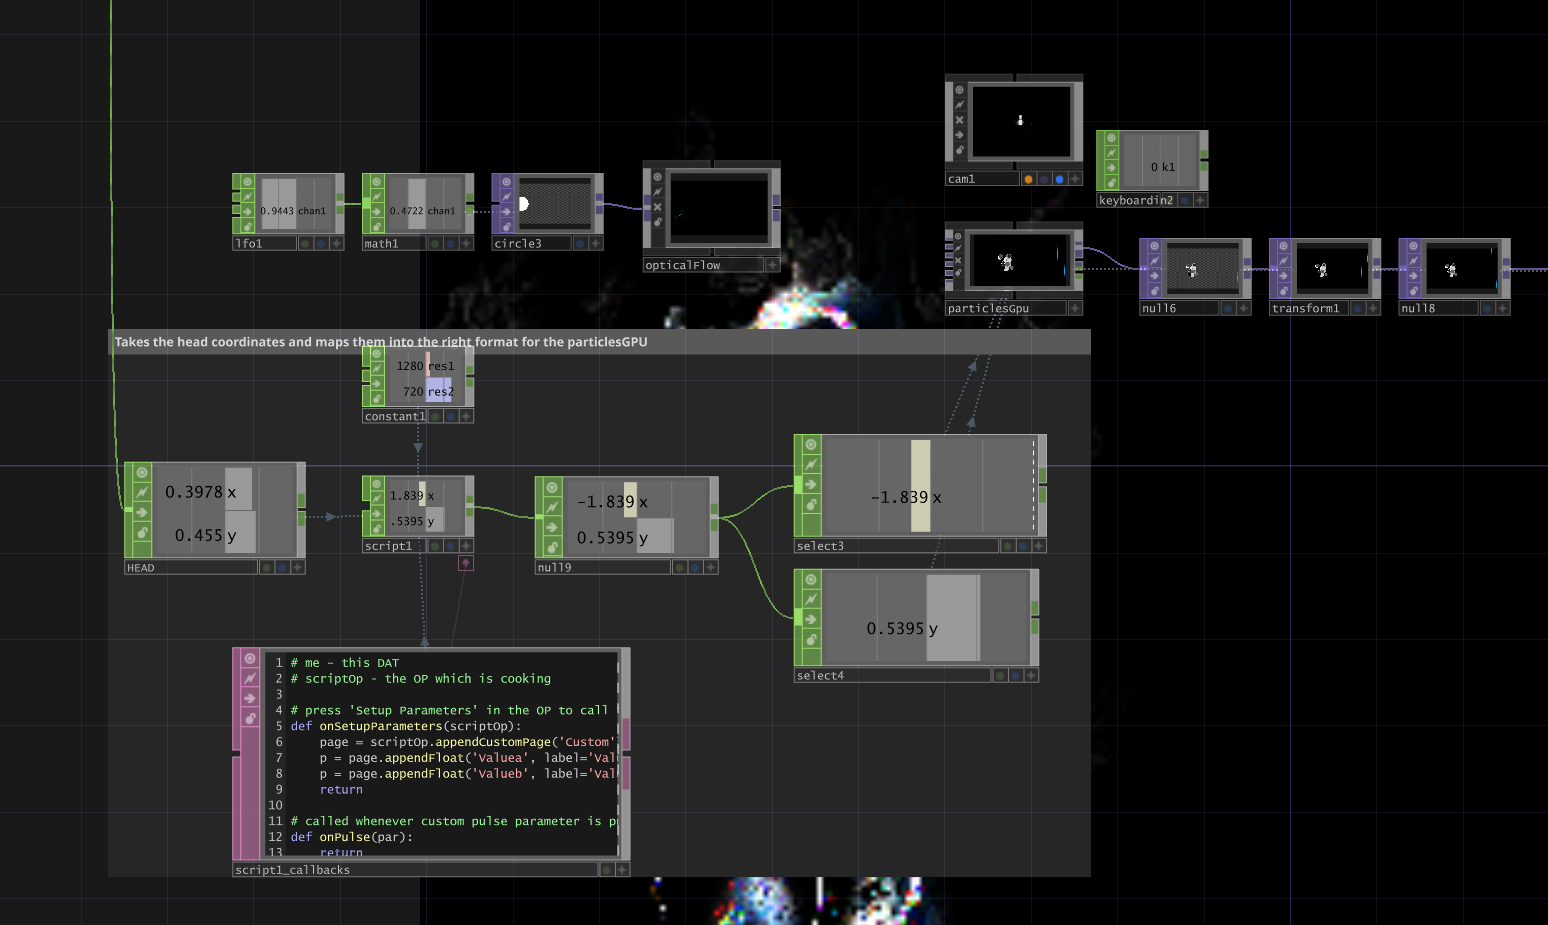
\includegraphics[width=0.8\textwidth]{images/docupictures/NoisyBlob_HEAD_to_ParticleGPU_Translate.png}
    \caption{Hand-Feuer-Implementation: ParticleGPU-basierte Echtzeit-Responsivität}
    \label{fig:hand_fire_system}
\end{figure}

\textbf{Implementation:} TouchDesigners ParticleGPU für blaue Flammenpartikel, extrahiert Hand-Landmarks (MediaPipe Nodes 15/16) und transformiert diese in normalisierte Bildschirmkoordinaten.

\textbf{Koordinaten-Transformation im Detail (PY\_NodeToParticleGPUtranslate.py):}
\begin{itemize}
    \item \textbf{Input:} MediaPipe normalisierte Koordinaten [0,1] vom HEAD-Operator
    \item \textbf{Remapping-Formel:} 
    \begin{itemize}
        \item X: \texttt{tdu.remap(x\_norm, 0.0, 1.0, -9.0, 9.0)}
        \item Y: \texttt{tdu.remap(y\_norm, 0.0, 1.0, 6.0, -6.0)} (invertiert für TouchDesigner)
    \end{itemize}
    \item \textbf{Koordinatenraum:} [-9, 9] horizontal, [-6, 6] vertikal für ParticleGPU-Weltkoordinaten
    \item \textbf{Resolution-Referenz:} constant1-TOP liefert Ausgabeauflösung (1920x1080)
    \item \textbf{Output:} CHOP-Kanäle 'x' und 'y' für direkte ParticleGPU-Force-Steuerung
\end{itemize}

\textbf{Produktionsergebnis:} Robuste Performance nach initialem Setup, fehlerfrei während gesamter Aufnahmezeit.

\subsubsection{Visual-System 2: Adaptive Kopfpartikel}

\textbf{Zustandsmaschine:} Hand-zu-Schulter-Positionsvergleich triggert Partikel-Modus-Wechsel mit Interpolationsfunktion für sanfte Übergänge.

\textbf{Koordinaten-Transformation für Visualisierungs-Modi (PY\_NodeXYzuCentralisedSOPTranslate.py):}
\begin{itemize}
    \item \textbf{Funktion:} Koordinaten-Transformation von normalized zu projection space für rechte Hand
    \item \textbf{Algorithm:} \texttt{x = x\_norm * width/height - 1; y = 0.5 - y\_norm}
    \item \textbf{Input:} \texttt{rechteHand} CHOP mit normalisierten Koordinaten
    \item \textbf{Usage:} SOP-Koordinaten-Mapping für 3D-Geometrie-Positionierung beim Wechsel zwischen Visualisierungs-Modi
    \item \textbf{Integration:} Ermöglicht präzise Partikel-Positionierung relativ zum Performer
\end{itemize}

\textbf{Technische Umsetzung der Zustandslogik (PY\_RelativeNodeValuesToBlended0and1Switch.py):}
\begin{itemize}
    \item \textbf{Vergleichsalgorithmus:} \texttt{logic = 1 if (ly < sy or ry < sy) else 0}
    \begin{itemize}
        \item sy: SpineBase Y-Koordinate (Referenzpunkt)
        \item ly/ry: Linke/Rechte Hand Y-Koordinate
    \end{itemize}
    \item \textbf{Animationssteuerung:} Zeitbasierte Interpolation mit absTime.seconds
    \item \textbf{Blend-Duration:} Dynamisch über blend\_param CHOP (Standard: 0.3s)
    \item \textbf{Interpolationsformel:} \texttt{anim\_value = start + (target - start) * t}
    \item \textbf{Switch-TOP Integration:} Direktes Schreiben auf switch1.par.index
\end{itemize}

\textbf{Produktionserfahrung:} Funktional, aber frontale Kamera-Beamer-Konstellation erfordert häufige Nachkalibrierung – arbeitsintensiv in Produktionsumgebung.

\subsubsection{Visual-System 3: 64-Spike Radialsystem}

\begin{figure}[h]
    \centering
    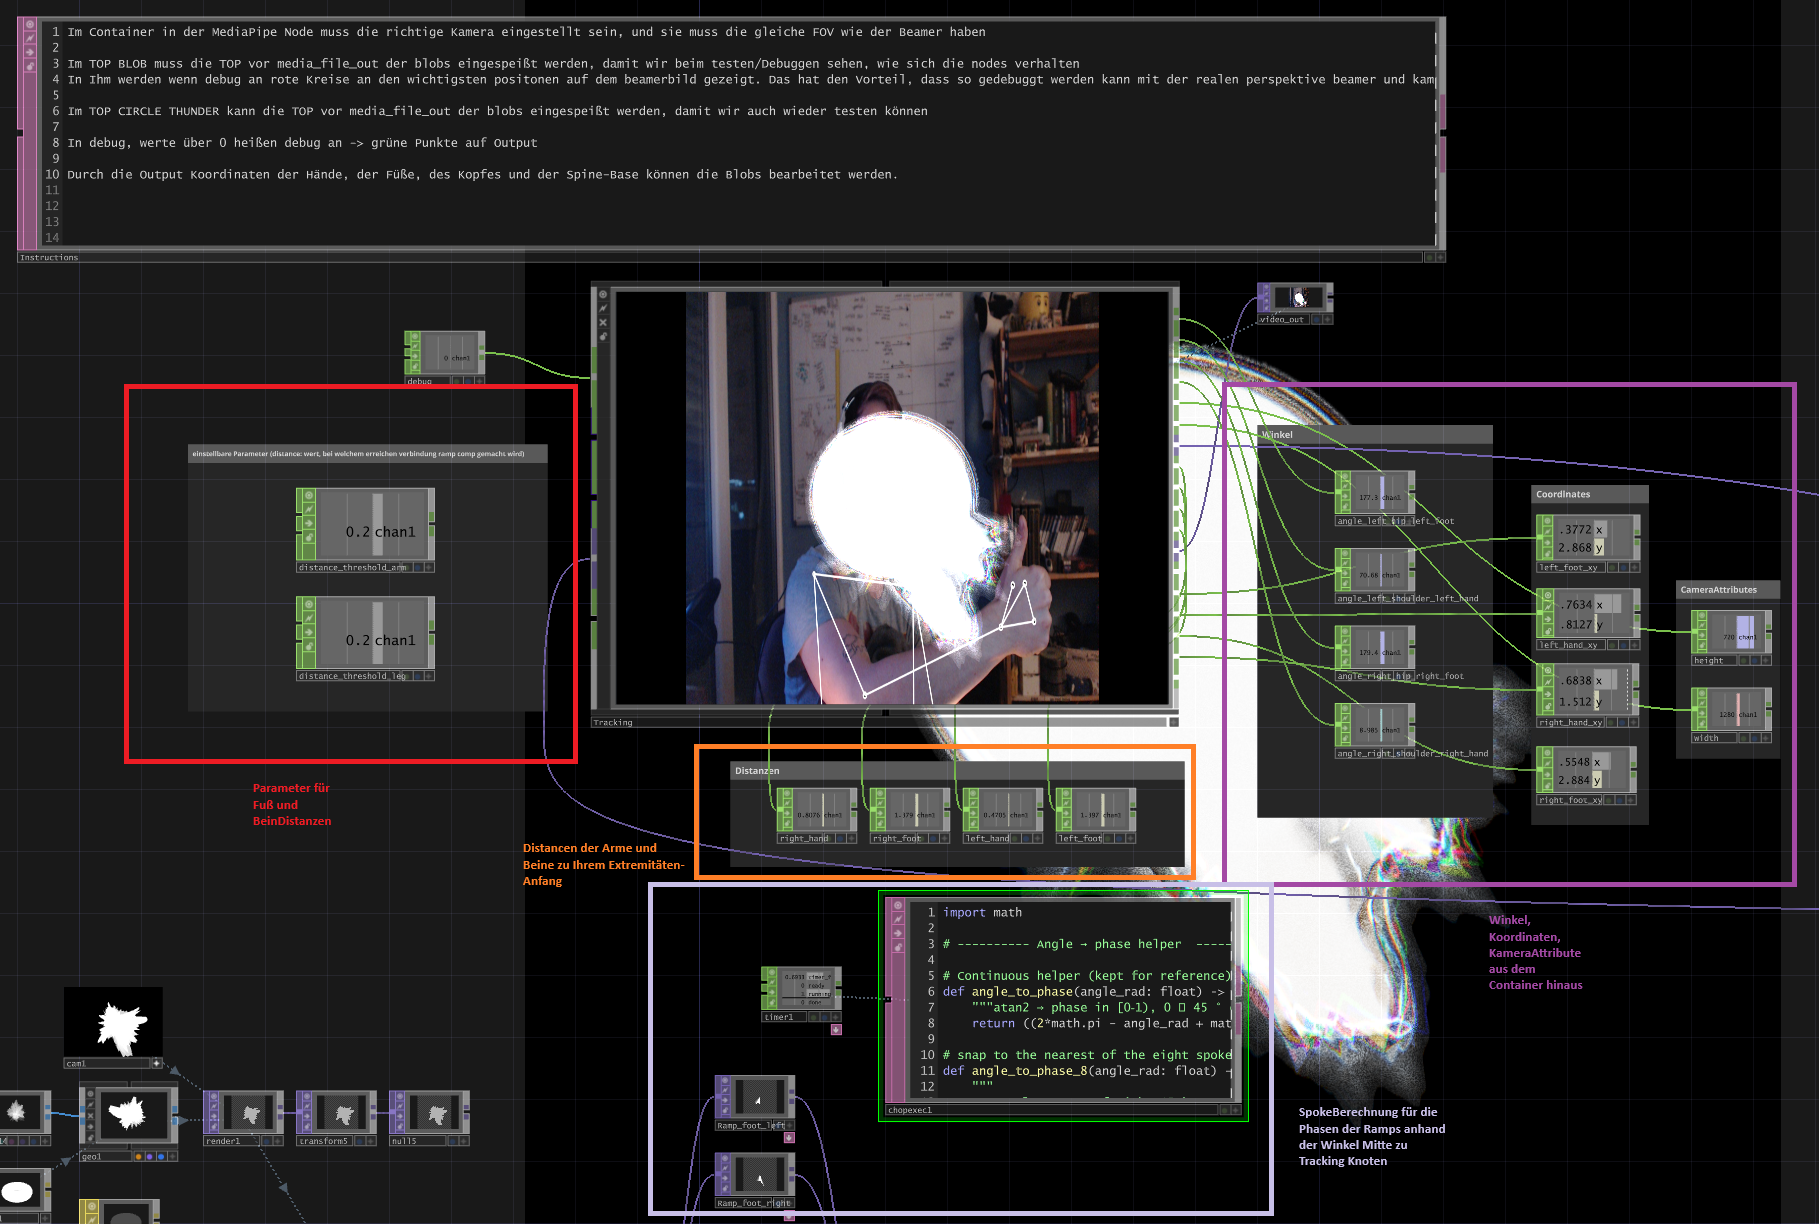
\includegraphics[width=0.8\textwidth]{images/docupictures/TopDown_KreisZuRampsParametisierteBerechnungen.png}
    \caption{64-Spike-System: Polar-Koordinaten-Mapping mit 5,625° Auflösung}
    \label{fig:spike_system_production}
\end{figure}

\textbf{Algorithmus:} atan2-basierte Polar-Koordinaten-Berechnung mappt Hand-/Fußpositionen auf diskrete Spike-Indizes (0-63) mit Intensitäts-Distanz-Korrelation.

\textbf{Detaillierte Polar-Koordinaten-Transformation (PY\_AngleToPhaseSkript):}
\begin{itemize}
    \item \textbf{Aspect-Ratio-Korrektur:} \texttt{x\_wide = x\_raw * aspect} für kreisförmige Distanzen
    \item \textbf{Zentrierung:} \texttt{dx = x\_wide - cx\_wide}, \texttt{dy = y - cy} (cx\_wide = 0.5 * aspect)
    \item \textbf{Polar-Konversion:} 
    \begin{itemize}
        \item \texttt{dist = math.hypot(dx, dy)}
        \item \texttt{angle = math.atan2(dy, dx)}
    \end{itemize}
    \item \textbf{Phase-Mapping (20-Spoke):} \texttt{angle\_to\_phase\_20(angle)}
    \begin{itemize}
        \item Basis: \texttt{((2*$\pi$ - angle + $\pi$/4) / (2*$\pi$)) \% 1.0}
        \item Diskretisierung: \texttt{idx = int(p * 20 + 0.5) \% 20}
        \item 18°-Schritte mit 0/20 = 45° (SE)
    \end{itemize}
    \item \textbf{Schwellenwert-Logik:} Dynamische Verbindung bei \texttt{dist >= threshold}
    \item \textbf{Ramp-TOP-Control:} Automatisches connect/disconnect zu comp15
\end{itemize}

\textbf{Produktionserfolg:} Optimale Performance bei Top-Down-Aufbau, vollständig fehlerfrei während gesamter Aufnahme – das zuverlässigste der drei Systeme.

\subsection{Produktionsvalidierung im Albrecht-Ade-Studio}

\textbf{Zweitägige Intensivtests unter realen Bedingungen:}

\textbf{Tag 1 - System-Integration und Setup-Optimierung:}
\begin{itemize}
    \item \textbf{Infrarot-Modi:} Problemlose Integration, keine Beleuchtungsinterferenzen
    \item \textbf{RGB-Modi:} Funktional unter kontrollierten Lichtbedingungen
    \item \textbf{Setup-Wechsel:} Unter 30 Minuten zwischen Visualisierungsmodi
    \item \textbf{Systemstabilität:} Null kritische Ausfälle während Produktionszeit
\end{itemize}

\textbf{Tag 2 - Vollständige Choreographie-Integration:}
\begin{itemize}
    \item \textbf{1,5 TB Footage:} Vollständige 4K-Aufnahme mit M.A.S.K.-Integration
    \item \textbf{45 Takes:} Kontinuierliche Tracking-Performance ohne Unterbrechungen
    \item \textbf{Professional Workflow:} Nahtlose Integration in Filmproduktions-Pipeline
\end{itemize}

\newpage

\subsection{Quantifizierte Performance-Metriken}

\begin{table}[H]
    \centering
    \begin{tabular}{|l|c|c|c|}
        \hline
        \textbf{System/Modus} & \textbf{Tracking-Genauigkeit} & \textbf{Setup-Aufwand} & \textbf{Produktionsstabilität} \\ \hline
        Top-Down Infrarot & Sehr hoch & Gering & Fehlerlos \\ \hline
        Frontale RGB & Mittel (lichtabhängig) & Hoch & Stabil mit Kalibrierung \\ \hline
        Hand-Feuer-System & Hoch (nach Setup) & Sehr gering & Robust \\ \hline
        64-Spike-System & Sehr hoch (Top-Down) & Minimal & Zuverlässig \\ \hline
        Adaptive Kopfpartikel & Gut (kalibrierungsabhängig) & Mittel & Arbeitsintensiv \\ \hline
    \end{tabular}
    \caption{Produktions-Performance-Vergleich der M.A.S.K.-Systeme}
    \label{tab:production_performance}
\end{table}

\subsection{Technische Lösungsbilanz}

\textbf{Erfolgreiche Lösungsansätze:}

\textbf{Infrarot-Adaptation:} Die spezifisch für Produktionsanforderungen angepasste Infrarot-MediaPipe-Pipeline adressiert effektiv das Problem der Beleuchtungsinterferenz – eine praxisorientierte Lösung mit direkter Produktionsrelevanz.

\textbf{Modulare TouchDesigner-Integration:} Container-basierte Architektur ermöglicht Plug-and-Play-Funktionalität und parallele Entwicklung verschiedener Visualisierungen.

\textbf{Performance-Optimierung:} Signifikante CPU-Nutzungsreduktion durch Systemvereinfachung und Architektur-Refactoring.

\textbf{Produktionserkenntnisse:}

\textbf{Top-Down-Überlegenheit:} Overhead-Tracking erwies sich als robuster und wartungsärmer als frontale Kamera-Setups.

\textbf{Infrarot-Immunität:} Vollständige Beleuchtungsunabhängigkeit ermöglicht kreative Freiheit bei Beamer-Intensität und -Effekten.

\textbf{Setup-Effizienz:} Kurze Setup-Zeiten erfüllen professionelle Produktionsanforderungen.

\subsection{Systemlimitationen und Scope}

\begin{itemize}
    \item \textbf{Single-Person-Tracking:} Bewusste Beschränkung auf einzelne Performer für Choreographie-Fokus.
    \item \textbf{Manuelle Kalibrierung:} Setup-Änderungen erfordern manuellen Kalibrierungsaufwand – akzeptabel für geplante Produktionsabläufe.
    \item \textbf{Hardware-Abhängigkeit:} Kinect V2 als einzige Infrarot-Quelle – robust und kostengünstig ($\approx$90€ gebraucht).
    \item \textbf{Positionierung vs. Konkurrenz:} M.A.S.K. konkurriert nicht mit professionellen Systemen wie OptiTrack, sondern schließt die Lücke zwischen Consumer-Hardware und Profi-Equipment für spezielle Anwendungen unter herausfordernden Beleuchtungsbedingungen.
\end{itemize}

Das M.A.S.K.-System demonstriert erfolgreich, wie constraints-driven engineering zu eleganten, produktionstauglichen Lösungen führt. Die Infrarot-Adaptation entstand aus praktischen Notwendigkeiten und beweist ihre Wirksamkeit durch fehlerfreie Performance unter realen Produktionsbedingungen.